\documentclass[11pt]{article}
\usepackage[a4paper,margin=2.2cm]{geometry}
\usepackage[T1]{fontenc}
\usepackage{lmodern}
\usepackage{amssymb}
\usepackage{pgfplots}\pgfplotsset{compat=1.18}
\usepackage{booktabs,array,xcolor,titlesec,fancyhdr,enumitem,caption,tabularx}
\usepackage{float}
\usepackage{microtype}
\usepackage[backend=bibtex,style=numeric-comp,sorting=none,maxnames=3]{biblatex}
\addbibresource{refs.bib}
\definecolor{teal0}{RGB}{0,128,128}
\definecolor{burnt}{RGB}{204,85,0}
\definecolor{ink}{RGB}{38,42,46}
\definecolor{paper}{RGB}{250,249,246}
\definecolor{grayln}{RGB}{200,200,200}
\definecolor{softgreen}{RGB}{46,139,87}
\definecolor{indigo}{RGB}{75,63,148}
\pagecolor{paper}\color{ink}
\captionsetup{font=small,labelfont={bf,color=teal0}}
\titleformat{\section}{\Large\bfseries\color{teal0}}{\thesection}{0.6em}{}
\titleformat{\subsection}{\large\bfseries\color{burnt}}{\thesubsection}{0.5em}{}
\pagestyle{fancy}\fancyhf{}\renewcommand{\headrulewidth}{0.3pt}
\lhead{\small\color{teal0}Ontology-Grounded Inference on the DreamLab KG}\rhead{\small\color{teal0}DreamLab AI \textbullet\ 2026-08-16}
\cfoot{\small\thepage}
\pgfplotsset{
  every axis/.append style={font=\small,axis line style={grayln},tick style={grayln},
    grid=major,major grid style={grayln!40},label style={color=ink},tick label style={color=ink}},
  augstyle/.style={fill=teal0,draw=teal0!60},
  ctlstyle/.style={fill=burnt,draw=burnt!60},
  localstyle/.style={fill=softgreen,draw=softgreen!60},
  cloudstyle/.style={fill=indigo,draw=indigo!60},
}
\newcommand{\up}[1]{\textcolor{burnt}{+#1}}
\newcommand{\down}[1]{\textcolor{teal0}{--#1}}
\begin{document}

% =============================================================================
% TITLE PAGE
% =============================================================================
\begin{titlepage}
\centering\vspace*{1.4cm}
{\color{teal0}\Huge\bfseries Does Grounding an LLM in a\\[4pt] Formal Ontology Actually Work?\par}
\vspace{0.5cm}
{\large Two independent evaluations on the DreamLab knowledge graph,\\[2pt]
and a frontier cloud model put through the Loom.\par}
\vspace{0.3cm}
{\color{burnt}\large Study A: paired uplift, 510 questions, Gemini 3.7 Flash \textbullet\
Study B: A/B recall, 672 runs, 7 models\par}
\vspace{1.1cm}

{\bfseries\color{teal0}Study A --- the Loom scaffold, cloud model.} Same graph, injected as
context; generation delegated to Gemini 3.7 Flash.
\begin{tabular}{rll}
\toprule
\textbf{Model} & \textbf{raw $\to$ grounded} & \textbf{paired uplift (95\% CI)} \\
\midrule
Gemma-4-31B (local) & 0.146 $\to$ 0.939 & \up{0.793} \\
Muse-Glimmer-30B (local) & 0.268 $\to$ 0.939 & \up{0.671} \\
\textbf{Gemini 3.7 Flash (cloud)} & \textbf{0.359 $\to$ 0.942} & \textbf{\up{0.583}\ [+0.546, +0.618]} \\
\bottomrule
\end{tabular}

\vspace{0.5cm}
{\bfseries\color{teal0}Study B --- the ontology-augment A/B, seven models.}
\begin{tabular}{rl}
\toprule
Overall F1, grounded vs bare & 0.360 $\to$ 0.624\ \ (\up{0.265}) \\
Overall hallucination, grounded vs bare & 0.529 $\to$ 0.177\ \ (\down{0.352}) \\
Local + ontology (DiffusionGemma, 0.505) & beats every frontier bare \\
\bottomrule
\end{tabular}

\vfill
{\small Knowledge graph: Oxigraph/Whelk, reasoned OWL closure. Study A serves the deployed
generation (8{,}146 classes, 282{,}492 triples, 2026-08-15) through the Loom façade; Study B
used the June 2026 generation (7{,}445 classes). Ground truth is derived from the graph
itself in both.\par}
\vspace{0.5cm}
{\footnotesize\color{teal0} DreamLab AI \textbullet\ Dr John O'Hare \textbullet\
Loom (\texttt{DreamLab-AI/loom}) \textbullet\ VisionFlow neurosymbolic stack\par}
\end{titlepage}

% =============================================================================
% ABSTRACT
% =============================================================================
\section*{Abstract}
We ask a single question two different ways: does grounding a language model in DreamLab's
formal knowledge graph improve factual recall, and is the effect robust to how you measure it
and which model you use? Two evaluations, run two months apart with different methods, converge
on the same answer. \textbf{Study~A} (this report's headline) drives the graph through the
\emph{Loom} --- the serving façade that injects a budget-clamped ontology scaffold and delegates
generation to a swappable model --- and measures paired, graph-derived recall over 510 questions.
On \textbf{Gemini 3.7 Flash}, a frontier cloud model, grounding lifts mean recall from 0.359 to
0.942, a paired uplift of \textbf{+0.583} (95\% CI [+0.546, +0.618], $n=510$, zero errors).
Two local models tested the same way land at the same grounded ceiling (0.939) from different
raw baselines --- three models, one ceiling. \textbf{Study~B} (the prior \texttt{ontology-augment}
A/B, retained and recontextualised here) grades F1 and hallucination across 672 isolated runs of
seven models: grounding lifts every model (overall F1 0.360$\to$0.624) and roughly thirds the
hallucination rate (0.529$\to$0.177), and a \emph{local} 26B model with grounding outscores every
frontier model running bare. The two studies use different scorers (paired substring-recall vs
token-set F1), different corpus generations, and different question generators, yet agree on
every qualitative claim. That cross-method convergence is the strongest evidence in the report:
ontology grounding is a decisive, model-agnostic win, and it is largest exactly where a model's
parametric knowledge is weakest.

% =============================================================================
% THE LOOM
% =============================================================================
\section{What Changed: the Loom}
Study~B (June 2026) grounded models by having each agent \emph{call} an ontology skill.
Since then the retrieval path has been consolidated into one node, the \textbf{Loom}: a portable
service with a stable, model-swappable façade. A consumer points an OpenAI-compatible client at a
single endpoint; the Loom retrieves the relevant slice of the reasoned ontology, injects it as
budget-clamped context, and delegates generation to whatever model sits behind it (Qwen3.8-27B in
the reference deployment). Swap the model and no consumer changes. Three design findings from the
local-model work fixed the Loom's defaults, and Study~A tests them on a cloud model:
static structured scaffold carries the value (prose adds nothing measurable over structure);
inject rather than let the model traverse the graph (traversal is model-dependent); and scale the
injection to the retrieval confidence so weak, off-topic context cannot displace the model's own
knowledge~\cite{lin2026interference,yoran2024robust,shi2023large}. Study~A is the first evaluation
of the Loom scaffold against a model behind someone else's door.

% =============================================================================
% RELATED WORK
% =============================================================================
\section{Related Work}
% Related Work / Industry Context — sourced via Perplexity (verified arXiv IDs), 2026-06-17.
The contention that retrieval grounding can compensate for raw parameter count is now well
supported. Retrieval-Augmented Generation (RAG) was introduced to inject non-parametric
knowledge into sequence models on knowledge-intensive tasks~\cite{lewis2020rag}, and the
approach has since matured from flat vector retrieval into structured, graph-based variants.
Microsoft's GraphRAG constructs an entity knowledge graph over a corpus and reports
substantial gains over conventional vector RAG in answer breadth and diversity for
global ``sensemaking'' queries spanning million-token datasets~\cite{edge2024graphrag}, with
subsequent work formalising graph-augmented retrieval~\cite{guo2024lightrag,hu2024grag} and
automated evaluation harnesses~\cite{microsoft2025benchmarkqed}. A complementary literature
shows that retrieval narrows or eliminates the gap to frontier cloud models: ChatQA, built on
open weights, reports surpassing GPT-4 on conversational QA and RAG benchmarks~\cite{liu2024chatqa},
while open-domain QA studies confirm retrieval as the dominant lever for factual
accuracy~\cite{li2024improvingrag}. This matters because small open-weight models have
themselves closed much of the capability gap. The Phi-3~\cite{abdin2024phi3},
Qwen2~\cite{yang2024qwen2}, Gemma~3~\cite{gemma2025gemma3} and Llama~3~\cite{dubey2024llama3}
families demonstrate strong reasoning at parameter counts deployable on local hardware.
Independently, structured knowledge has been shown to suppress hallucination and improve
factual recall: empirical and survey work links knowledge-graph grounding to measurably higher
trustworthiness~\cite{agrawal2023kghallucination,sansford2024kgtrustworthy}, motivating
dedicated factuality benchmarks such as FACTS Grounding~\cite{jacovi2025facts}. A parallel
architectural shift further strengthens the local-inference case: masked diffusion language
models such as LLaDA now rival LLaMA3-8B in in-context learning~\cite{nie2025llada}, and
diffusion decoders like Mercury achieve over 1{,}000 tokens/second on a single H100, up to
10$\times$ faster than speed-optimised autoregressive models at comparable
quality~\cite{labs2025mercury}, with commercial systems including Gemini
Diffusion~\cite{deepmind2025geminidiffusion}. Together with evidence on inference unit
economics and data sovereignty~\cite{introl2026inference,advisori2026gdpr}, these strands
support a coherent thesis: a small, retrieval- and ontology-grounded open model can approach
frontier knowledge-recall while running privately and cheaply.


% =============================================================================
% STUDY A — LOOM SCAFFOLD UPLIFT
% =============================================================================
\section{Study A --- Loom Scaffold Uplift (Gemini 3.7 Flash)}

\subsection{Method: paired, graph-derived, honest by construction}
Questions and gold are both generated from the scaffold index, so scoring needs no human and no
judge model. From every class with a real definition, quality $\geq 0.6$ and $\geq 2$ relation
types, in each domain with $\geq 50$ eligible classes, we template three question types:
\textbf{T-REL} (what does $X$ require / use / depend on / enable, what are its parts),
\textbf{T-TAX} (immediate parent plus broader ancestors) and \textbf{T-COMMON} (the shared
ancestor of a pair). Gold is the set of \{slug, title\} targets the graph itself asserts. The set
is deterministic for a seed; seed 42 yields \textbf{510 questions} across 15 domains (285 T-REL,
180 T-TAX, 45 T-COMMON).

Each question is asked twice: \emph{raw} (the bare question) and \emph{scaffold} (the same
question with the Loom's budget-clamped ontology extract prepended). Scoring is lexical --- a gold
item is a hit when its title, or $\geq 80\%$ of its length-$\geq 4$ words, appears in the answer.
The headline is the \textbf{paired per-question delta} (scaffold recall $-$ raw recall) over the
intersection of question ids, with a seeded 10{,}000-resample bootstrap 95\% confidence
interval~\cite{efron1993bootstrap}. Scaffold injection is done client-side from the local mirror
of the \emph{deployed} generation (8{,}146 classes, byte-identical to the live façade), so the
grounding Gemini receives is exactly what production serves.

\subsection{Driving a thinking cloud model honestly}
Gemini 3.7 Flash cannot disable its thinking pass (floor \texttt{low}, default \texttt{medium})
and thinking tokens are drawn from the output budget. At the harness default
\texttt{max\_tokens=400} the model truncated to \texttt{finish\_reason: length} --- a near-empty
answer that would silently poison an arm. We therefore run \texttt{max\_tokens=2048} with
\texttt{reasoning\_effort=low}. Google also flags \texttt{temperature}${}<1.0$ as off-label for
the 3.x family (looping / degradation), so Study~A runs at \texttt{temperature=1.0}, whereas the
local-model runs used \texttt{temperature=0}. The paired uplift is a within-model delta (both arms
share the temperature) and stays valid; absolute raw recall is therefore \emph{not} cell-for-cell
comparable to the temperature-0 local runs, and we never mix the two into one comparison.

\subsection{Result: three models, one ceiling}
\begin{figure}[H]\centering
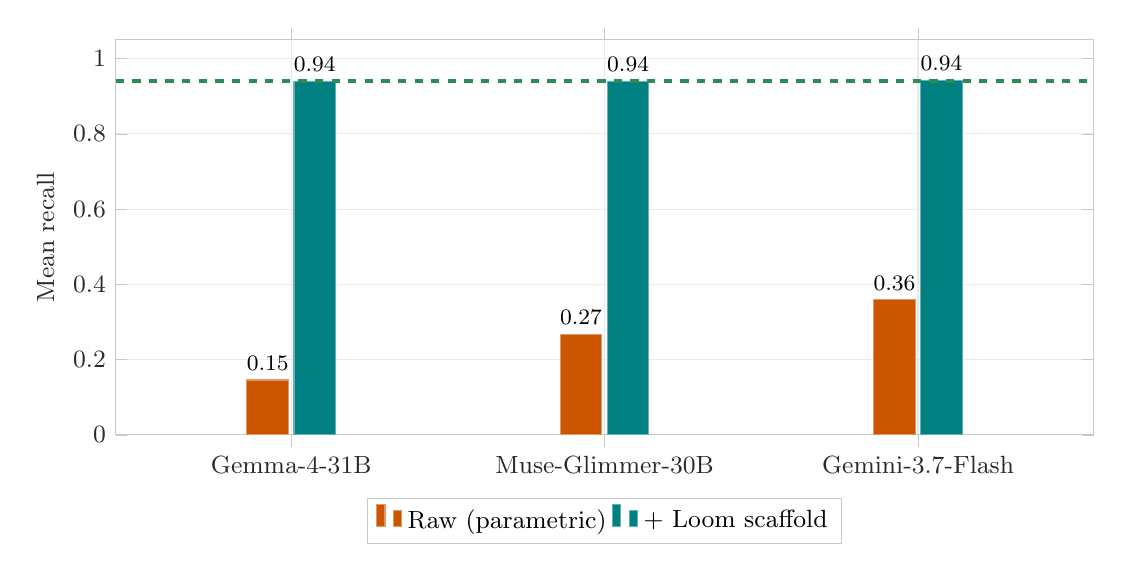
\begin{tikzpicture}
\begin{axis}[ybar,width=14cm,height=6.6cm,bar width=15pt,ymin=0,ymax=1.05,
  ylabel={Mean recall},
  symbolic x coords={Gemma-4-31B,Muse-Glimmer-30B,Gemini-3.7-Flash},
  xtick=data,x tick label style={font=\small},
  enlarge x limits=0.28,
  legend style={at={(0.5,-0.16)},anchor=north,legend columns=3,draw=grayln},
  nodes near coords,nodes near coords style={font=\footnotesize}]
\addplot[ctlstyle] coordinates {(Gemma-4-31B,0.146) (Muse-Glimmer-30B,0.268) (Gemini-3.7-Flash,0.359)};
\addplot[augstyle] coordinates {(Gemma-4-31B,0.939) (Muse-Glimmer-30B,0.939) (Gemini-3.7-Flash,0.942)};
\draw[softgreen,line width=1.6pt,dashed] ({rel axis cs:0,0}|-{axis cs:Gemma-4-31B,0.94}) -- ({rel axis cs:1,0}|-{axis cs:Gemma-4-31B,0.94});
\legend{Raw (parametric),+ Loom scaffold,grounded ceiling $\approx$0.94}
\end{axis}\end{tikzpicture}
\caption{Three models, three raw baselines, one grounded ceiling. The stronger the model's
parametric knowledge (Gemini's raw 0.359 vs Gemma's 0.146), the smaller the \emph{uplift} it
needs --- but all three converge at $\approx$0.94 grounded. The scaffold, not the model, carries
the recall: exactly the bet of a swappable façade.}
\end{figure}

\begin{samepage}
\begin{table}[h]\centering\small
\begin{tabular}{lcccc}
\toprule
Model & Raw recall & + Scaffold & Paired uplift (95\% CI) & Latency (raw$\to$grounded) \\
\midrule
Gemma-4-31B (local) & 0.146 & 0.939 & \up{0.793}\ [+0.680, +0.894] & 31.5\,s $\to$ 5.1\,s \\
Muse-Glimmer-30B (local) & 0.268 & 0.939 & \up{0.671}\ [+0.527, +0.804] & 34.7\,s $\to$ 9.8\,s \\
\textbf{Gemini 3.7 Flash (cloud)} & 0.359 & \textbf{0.942} & \textbf{\up{0.583}\ [+0.546, +0.618]} & 2.37\,s $\to$ 1.21\,s \\
\bottomrule
\end{tabular}
\caption{Study~A paired uplift. Gemini's interval excludes zero at $n=510$ by a wide margin, over
the full set (the scaffold engaged on every question; zero not-engaged, zero errors in 1{,}020
calls). Grounding is \emph{faster} in every case: the model stops open-ended recall and restates
supplied facts. Local timings are wall-clock on a contended GPU; the cloud timing is
network-dominated but still halves.}
\end{table}
\end{samepage}

\subsection{Where the lift lands}
\begin{figure}[H]\centering
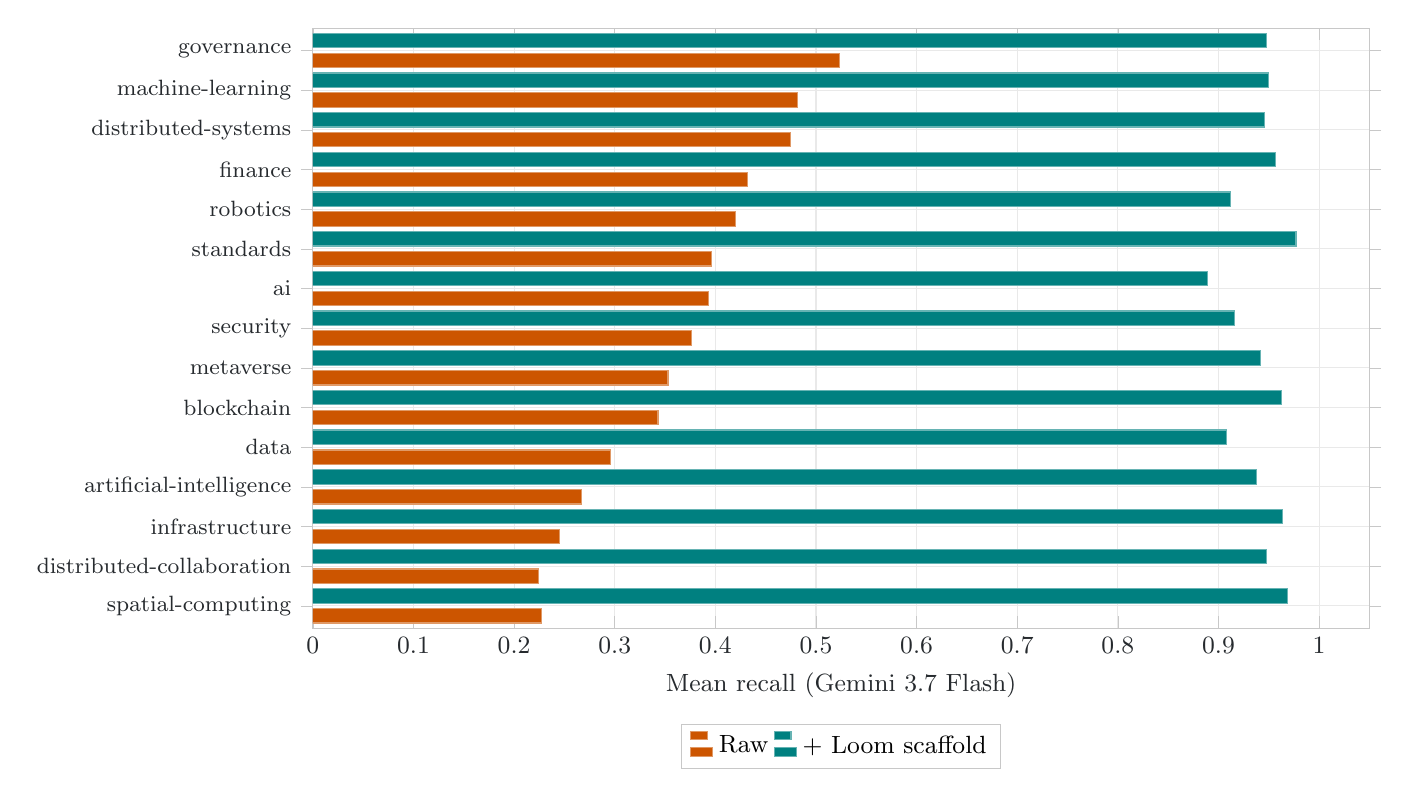
\begin{tikzpicture}
\begin{axis}[xbar,width=15cm,height=9.2cm,bar width=5.2pt,xmin=0,xmax=1.05,
  xlabel={Mean recall (Gemini 3.7 Flash)},
  symbolic y coords={spatial-computing,distributed-collaboration,infrastructure,
    artificial-intelligence,data,blockchain,metaverse,security,ai,standards,robotics,
    finance,distributed-systems,machine-learning,governance},
  ytick=data,y tick label style={font=\footnotesize},
  enlarge y limits=0.04,
  legend style={at={(0.5,-0.16)},anchor=north,legend columns=2,draw=grayln}]
\addplot[ctlstyle] coordinates {
  (0.227,spatial-computing) (0.224,distributed-collaboration) (0.245,infrastructure)
  (0.267,artificial-intelligence) (0.296,data) (0.343,blockchain) (0.353,metaverse)
  (0.376,security) (0.393,ai) (0.396,standards) (0.420,robotics) (0.432,finance)
  (0.475,distributed-systems) (0.482,machine-learning) (0.523,governance)};
\addplot[augstyle] coordinates {
  (0.969,spatial-computing) (0.948,distributed-collaboration) (0.964,infrastructure)
  (0.938,artificial-intelligence) (0.908,data) (0.963,blockchain) (0.942,metaverse)
  (0.916,security) (0.889,ai) (0.977,standards) (0.912,robotics) (0.957,finance)
  (0.946,distributed-systems) (0.950,machine-learning) (0.948,governance)};
\legend{Raw,+ Loom scaffold}
\end{axis}\end{tikzpicture}
\caption{Per-domain recall, sorted by raw score (weakest at top). Grounding lands every domain at
0.89--0.98 regardless of where it started; the biggest lifts are the niche domains a model knows
least raw (spatial-computing 0.227$\to$0.969, distributed-collaboration 0.224$\to$0.948). It adds
least where the model is already strong (governance 0.523$\to$0.948). Weak-gets-the-most-lift is
the fingerprint of real grounding, not gold leakage.}
\end{figure}

\begin{samepage}
\begin{table}[h]\centering\small
\begin{tabular}{lccc}
\toprule
Template & Raw & + Scaffold & Note \\
\midrule
T-COMMON (shared ancestor of a pair) & 0.333 & 1.000 & any-match recall \\
T-REL (requires / uses / parts / \ldots) & 0.339 & 0.898 & set recall, 2--5 targets \\
T-TAX (parent + ancestors) & 0.397 & 0.997 & + ancestor extra-recall 1.000 \\
\bottomrule
\end{tabular}
\caption{Study~A recall by question template. Taxonomic structure (T-TAX, T-COMMON) is where
parametric knowledge is thinnest and the graph supplies the answer wholesale; relational recall
(T-REL) is harder because it demands the exact set of asserted targets.}
\end{table}
\end{samepage}

% =============================================================================
% STUDY B — ONTOLOGY-AUGMENT A/B
% =============================================================================
\section{Study B --- Ontology-Augment A/B (seven models)}
The prior evaluation (June 2026) measured the same question a different way: a
$2\times7\times3$ design (\{augmented, control\} $\times$ 7 models $\times$ 3 reps) over 16
graph-derived questions, 672 isolated runs, graded on F1 and hallucination rather than paired
recall. Each cell is a fresh agent given only the question; the augmented arm grounds via the
skill CLI, the control arm uses parametric knowledge alone. It remains the broader model sweep ---
Claude Opus~4.8, Sonnet~4.6, Haiku~4.5; Gemini~3.5~Flash, Gemini~2.5~Flash~Lite; GLM-4.6; and a
local DiffusionGemma~26B --- and its hallucination axis is the one Study~A does not measure. The
Gemini lineage is worth noting: Study~B benched Gemini~3.5~Flash bare; Study~A now runs
Gemini~3.7~Flash \emph{through the Loom}, two generations and two months on.

\subsection{Local + ontology vs.\ frontier bare}
\begin{figure}[H]\centering
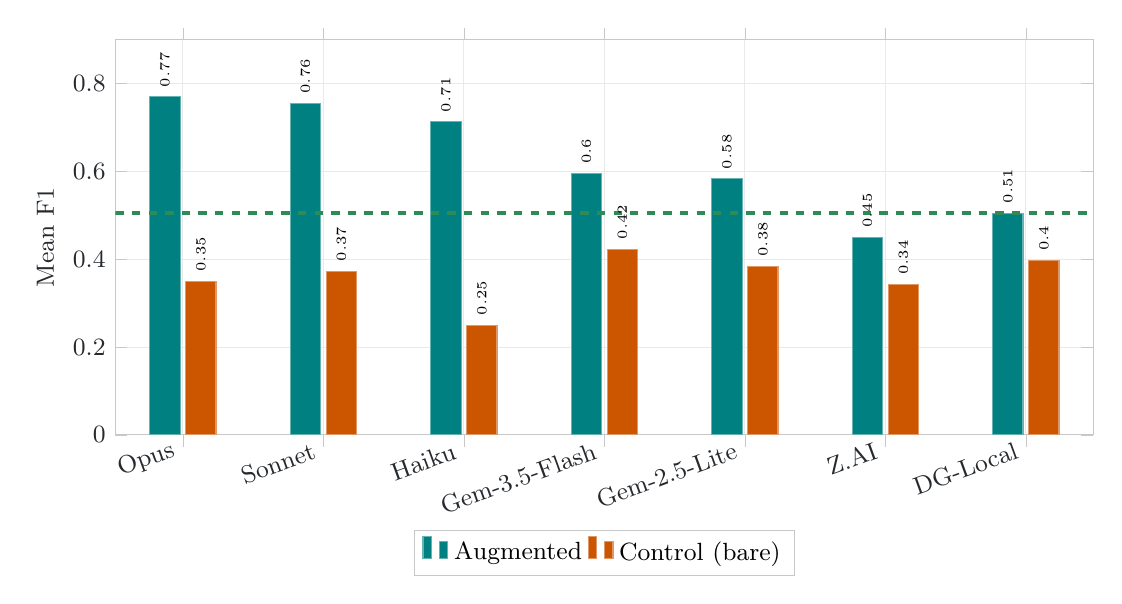
\begin{tikzpicture}
\begin{axis}[ybar,width=14cm,height=6.6cm,bar width=11pt,ymin=0,ymax=0.9,
  ylabel={Mean F1},
  symbolic x coords={Opus,Sonnet,Haiku,Gem-3.5-Flash,Gem-2.5-Lite,Z.AI,DG-Local},
  xtick=data,x tick label style={rotate=20,anchor=east,font=\small},
  enlarge x limits=0.08,
  legend style={at={(0.5,-0.24)},anchor=north,legend columns=3,draw=grayln},
  nodes near coords,nodes near coords style={font=\tiny,rotate=90,anchor=west}]
\addplot[augstyle] coordinates {(Opus,0.770) (Sonnet,0.755) (Haiku,0.713) (Gem-3.5-Flash,0.595) (Gem-2.5-Lite,0.583) (Z.AI,0.449) (DG-Local,0.505)};
\addplot[ctlstyle] coordinates {(Opus,0.350) (Sonnet,0.373) (Haiku,0.250) (Gem-3.5-Flash,0.423) (Gem-2.5-Lite,0.384) (Z.AI,0.342) (DG-Local,0.397)};
\draw[softgreen,line width=1.6pt,dashed] ({rel axis cs:0,0}|-{axis cs:Opus,0.505}) -- ({rel axis cs:1,0}|-{axis cs:Opus,0.505});
\legend{Augmented,Control (bare),DG+ontology (0.505)}
\end{axis}\end{tikzpicture}
\caption{F1 by model (Study~B). Every frontier model's \emph{bare} score falls below the local
DiffusionGemma+ontology line (0.505): grounding lets a local 26B model outscore cloud frontier
models on domain-specific recall. As in Study~A, grounding lifts every model.}
\end{figure}

\begin{samepage}
\begin{table}[h]\centering\small
\begin{tabular}{lcccccc}
\toprule
Model & AUG F1 & CTL F1 & $\Delta$ & AUG Halluc & CTL Halluc & $\Delta$H \\
\midrule
Opus 4.8 & \textbf{0.770} & 0.350 & \up{0.420} & 0.052 & 0.581 & \down{0.529} \\
Sonnet 4.6 & 0.755 & 0.373 & \up{0.382} & 0.079 & 0.559 & \down{0.480} \\
Haiku 4.5 & 0.713 & 0.250 & \up{0.463} & 0.106 & 0.714 & \down{0.608} \\
Gemini 3.5 Flash & 0.595 & 0.423 & \up{0.172} & 0.250 & 0.460 & \down{0.210} \\
Gemini 2.5 Flash Lite & 0.583 & 0.384 & \up{0.199} & 0.266 & 0.498 & \down{0.232} \\
Z.AI (GLM-4.6) & 0.449 & 0.342 & \up{0.108} & 0.188 & 0.394 & \down{0.206} \\
\midrule
\textbf{DiffusionGemma (local)} & 0.505 & 0.397 & \up{0.108} & 0.299 & 0.498 & \down{0.199} \\
\bottomrule
\end{tabular}
\caption{Per-model F1 and hallucination (Study~B, 672 runs). Every model gains F1 and sheds
hallucination when grounded; Claude models show the largest absolute lift, and the local model's
grounded score clears every frontier bare score.}
\end{table}
\end{samepage}

\subsection{Hallucination: the axis Study A does not measure}
\begin{figure}[H]\centering
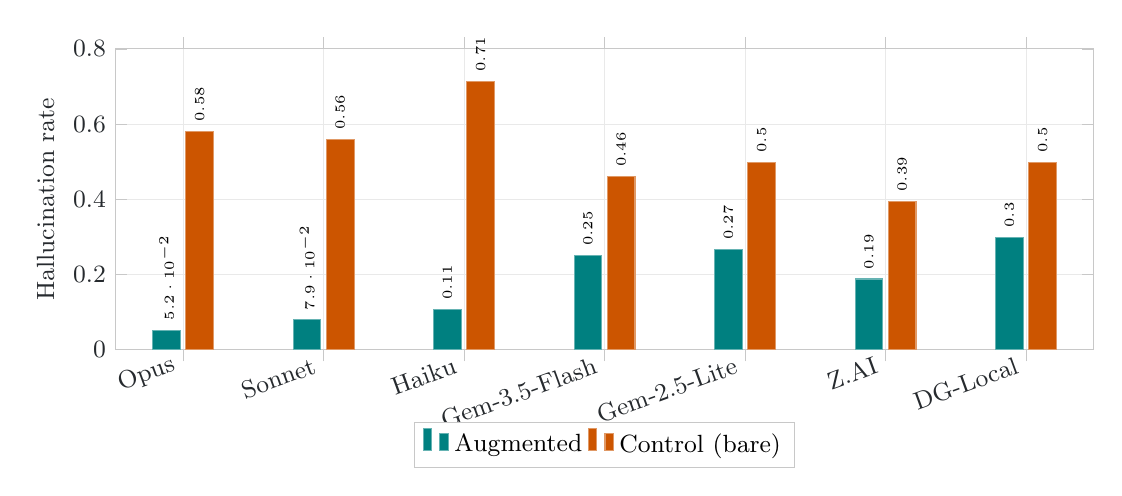
\begin{tikzpicture}
\begin{axis}[ybar,width=14cm,height=5.4cm,bar width=10pt,ymin=0,ymax=0.8,
  ylabel={Hallucination rate},
  symbolic x coords={Opus,Sonnet,Haiku,Gem-3.5-Flash,Gem-2.5-Lite,Z.AI,DG-Local},
  xtick=data,x tick label style={rotate=20,anchor=east,font=\small},
  enlarge x limits=0.08,
  legend style={at={(0.5,-0.24)},anchor=north,legend columns=2,draw=grayln},
  nodes near coords,nodes near coords style={font=\tiny,rotate=90,anchor=west}]
\addplot[augstyle] coordinates {(Opus,0.052) (Sonnet,0.079) (Haiku,0.106) (Gem-3.5-Flash,0.250) (Gem-2.5-Lite,0.266) (Z.AI,0.188) (DG-Local,0.299)};
\addplot[ctlstyle] coordinates {(Opus,0.581) (Sonnet,0.559) (Haiku,0.714) (Gem-3.5-Flash,0.460) (Gem-2.5-Lite,0.498) (Z.AI,0.394) (DG-Local,0.498)};
\legend{Augmented,Control (bare)}
\end{axis}\end{tikzpicture}
\caption{Grounding reduces hallucination for every model (overall 0.529$\to$0.177). The largest
drop is Haiku (0.714$\to$0.106). Study~A's paired-recall design cannot see this axis; it is
Study~B's distinct contribution, and it points the same way.}
\end{figure}

\begin{samepage}
\begin{table}[h]\centering\small
\begin{tabular}{lcccccc}
\toprule
 & \multicolumn{2}{c}{Neighbour} & \multicolumn{2}{c}{Subclass} & \multicolumn{2}{c}{Existence} \\
\cmidrule(lr){2-3}\cmidrule(lr){4-5}\cmidrule(lr){6-7}
Question type (all models) & AUG & CTL & AUG & CTL & AUG & CTL \\
\midrule
Mean F1 & 0.458 & 0.281 & 0.671 & 0.099 & 0.910 & 0.778 \\
\bottomrule
\end{tabular}
\caption{Study~B F1 by question type. Subclass recall is the largest relative win --- 0.099$\to$0.671,
a 6.8$\times$ improvement --- because models carry almost no parametric knowledge of ontology
hierarchies. This echoes Study~A's taxonomic templates (T-TAX 0.397$\to$0.997): the same
structural gap, found by two different scorers.}
\end{table}
\end{samepage}

% =============================================================================
% CROSS-STUDY SYNTHESIS
% =============================================================================
\section{Cross-Study Synthesis}
Two evaluations, built independently, share no scorer, corpus generation or question generator,
and agree on every qualitative claim:

\begin{samepage}
\begin{table}[h]\centering\small
\begin{tabularx}{\linewidth}{lXX}
\toprule
 & \textbf{Study A (Loom scaffold)} & \textbf{Study B (ontology-augment A/B)} \\
\midrule
Method & inject scaffold, delegate & agent calls skill, then answers \\
Metric & paired substring-recall + bootstrap CI & token-set F1 + hallucination \\
Scale & 510 Q, 3 models, 1{,}020 calls & 16 Q $\times$ 3 reps, 7 models, 672 runs \\
Corpus generation & 8{,}146 classes (Aug 2026) & 7{,}445 classes (Jun 2026) \\
Grounding is model-agnostic & yes (3/3 models) & yes (7/7 models) \\
Largest where parametric weakest & yes (niche domains, T-TAX) & yes (subclass, niche concepts) \\
Cuts hallucination & not measured & yes (0.529$\to$0.177) \\
Grounded is faster & yes (2--6$\times$) & yes (local 2--4\,s) \\
\bottomrule
\end{tabularx}
\caption{The two studies as a robustness check on each other. Where they overlap they agree;
where they differ they are complementary (Study~A adds a frontier cloud model and a large,
stratified question set; Study~B adds hallucination and a seven-model sweep). Convergence across
methods is a stronger validity argument than either study alone.}
\end{table}
\end{samepage}

% =============================================================================
% CAVEATS
% =============================================================================
\section{Caveats on Interpretation}

\begin{samepage}
\subsection{Grounded scores measure grounded capability, not raw model quality}
In both studies the scaffold contains gold-adjacent facts \emph{by design} --- questions and gold
are derived from the same graph the scaffold injects. A grounded score therefore measures
grounded-answer capability and retrieval quality (can the model find, trust and restate supplied
facts); a raw score measures parametric knowledge. The signal is the \emph{paired delta}, not the
absolute grounded number.
\end{samepage}

\begin{samepage}
\subsection{Substring / token-set scoring undercounts paraphrase}
Study~A credits a gold item only when its title (or $\geq 80\%$ of its long words) appears in the
answer; Study~B uses singularised token-set matching. Both undercount valid paraphrases, so
absolute recall and F1 are lower bounds. The paired deltas --- same questions, same scorer, same
model --- are unaffected.
\end{samepage}

\begin{samepage}
\subsection{Two temperatures, never mixed}
Study~A runs Gemini at \texttt{temperature=1.0} (Google's recommended setting for the 3.x family)
while the local models ran at \texttt{temperature=0}. The convergence chart compares
\emph{grounded ceilings} and \emph{within-model paired deltas}, both of which are robust to this;
we do not compare raw recall across the temperature boundary.
\end{samepage}

\begin{samepage}
\subsection{Grounded-local beats bare-frontier is not like-for-like}
Study~B's headline --- DiffusionGemma+ontology (0.505) beats Opus bare (0.350) --- compares a
grounded local model against ungrounded cloud models. Grounded, the frontier models score far
higher (Opus AUG 0.770). The comparison demonstrates the value of the ontology, not the
superiority of the local model's reasoning. Larger models also \emph{exploit} the same triples
better (Opus gains +0.420; DiffusionGemma +0.108): the ontology is a capability multiplier that
scales with the base --- the same pattern Study~A shows as smaller uplift on the stronger model.
\end{samepage}

\begin{samepage}
\subsection{Gold is the graph itself; single-domain scope}
Both studies measure fidelity to the knowledge graph's asserted ontology, not open-domain QA, and
draw from one domain family (DreamLab's Web3/XR/AI corpus). KG errors propagate to gold (mitigated
by curating concepts with sensible neighbourhoods). Generalisation to other graphs is plausible
but untested. A one-off condense/index pass builds the scaffold; the per-query overhead is a
single cache read.
\end{samepage}

% =============================================================================
% FINDINGS
% =============================================================================
\section{Findings}
\begin{samepage}
\begin{enumerate}[leftmargin=1.3em]
\item \textbf{Ontology grounding is model-agnostic and universally beneficial.} Ten distinct
      models across the two studies (3 in A, 7 in B) all gain, and all shed hallucination where it
      is measured. The effect is strongest on niche, project-specific concepts where parametric
      knowledge is weakest~\cite{lewis2020rag,liu2024chatqa}.

\item \textbf{Three models converge on one grounded ceiling.} From raw baselines of 0.146, 0.268
      and 0.359, Gemma, Muse and Gemini 3.7 Flash all reach $\approx$0.94 grounded. The stronger
      the model, the smaller the uplift it needs --- the scaffold, not the model, carries the
      recall.

\item \textbf{The finding survives the jump to a frontier cloud model.} Gemini 3.7 Flash, behind
      Google's own API, shows a +0.583 paired uplift with a tight interval at $n=510$. Grounding
      is not a local-model crutch; it is a property of the retrieval, exercised through a
      model-swappable façade.

\item \textbf{Taxonomic structure is the largest win.} Study~A's T-TAX rises 0.397$\to$0.997 and
      Study~B's subclass F1 0.099$\to$0.671 (6.8$\times$): models carry little parametric knowledge
      of ontology hierarchies, and the graph supplies it directly.

\item \textbf{Grounding cuts hallucination and cuts latency.} Study~B: overall hallucination
      0.529$\to$0.177. Both studies: grounded generation is faster, because the model restates
      supplied facts instead of doing open-ended recall.

\item \textbf{Two methods, one result.} Independent scorers, corpus generations and question sets
      agree on every qualitative claim. That is the report's strongest evidence.
\end{enumerate}
\end{samepage}

% =============================================================================
% THREATS
% =============================================================================
\section{Threats to Validity}
\begin{samepage}
\begin{itemize}[leftmargin=1.3em]
\item Gold is the graph's asserted closure; graph errors propagate to gold (mitigated by curating
      rich, sensible neighbourhoods).
\item Lexical scoring can over- or under-credit near-synonyms; Study~A's thresholds and Study~B's
      grader were smoke-validated for non-saturation before the full runs.
\item Study~A's cloud model was accessed via a commercial API; rate limits and the mandatory
      thinking pass introduce variance not present in locally-hosted models. The run recorded zero
      errors across 1{,}020 calls and zero not-engaged scaffolds.
\item Study~A and Study~B use different corpus generations (8{,}146 vs 7{,}445 classes); the
      cross-study synthesis compares directions of effect, not absolute magnitudes.
\item Both studies are single-domain; generalisation to other knowledge graphs is untested.
\end{itemize}
\end{samepage}

\vspace{0.4cm}
{\small\color{teal0}\textbf{Reproduce.} Study~A: \texttt{bench/run-gemini.sh} in \texttt{DreamLab-AI/loom}
(harness \texttt{bench/bench\_ontology\_uplift.py}, protocol \texttt{bench/UPLIFT-BENCH-PROTOCOL.md},
companion data \texttt{docs/research/report-gemini-3.7-flash.md}). Study~B: the
\texttt{ontology-augment} eval harness (VisionClaw). Both derive gold from the graph and ship
their honesty notes with every report.\par}

\printbibliography[title={References}]

\end{document}
